\chapter{Résultats}
\chaptermark{Résultats}
\label{chapter:resultats}
	
	\section{Introduction}

		Nous avons désormais implémenté tous les éléments de notre simulateur, et nous allons donc pouvoir à présent tester le bon fonctionnement de notre système complet. Cela va nous permettre de tester que les différentes briques logicielles s'interfacent bien toutes ensemble et que le simulateur a un comportement physique correct.
		
		Dans un premier temps, nous allons vérifier que le système respecte les exigences présentées dans le \textsc{Chapitre}~\ref{chapitre:systeme}, ainsi que le comportement des robots et de l'environnement développés dans les \textsc{Chapitre}~\ref{chapitre:environnement} et \textsc{Chapitre}~\ref{chapitre:robots}.

		Ensuite, nous nous pencherons sur la comparaison du simulateur avec des expérimentations faites avec les \gls{ROV}s \argos{} et \atoll{}, afin de déterminer si les résultats de simulations sont proches du comportement réel des robots, et si ce système permettrait bien de réduire les temps de développements en réduisant le nombre d'essais en conditions réelles à réaliser pour valider de nouvelles fonctionnalités.

	\section{Respect des exigences}

		\subsection{Introduction}

			Nous allons vérifier que notre système respecte bien les exigences présentées dans le \textsc{Chapitre}~\ref{chapitre:systeme}.

		\subsection{Visualisation des robots}

			\gls{ROS2} propose \textit{RViz2} qui est un outil qui permettant de visualiser les robots et les données fournies par les capteurs. Il est systématique de retrouver dans les packages de description de robots pour \gls{ROS2} un fichier de configuration permettant de visualiser le robot dans \textit{RViz2}. Pour notre simulateur, cela correspond à la fonction contrainte \textbf{FC3}.

			\begin{figure}
				\centering
				\begin{subfigure}[t]{0.45\textwidth}
					\centering
					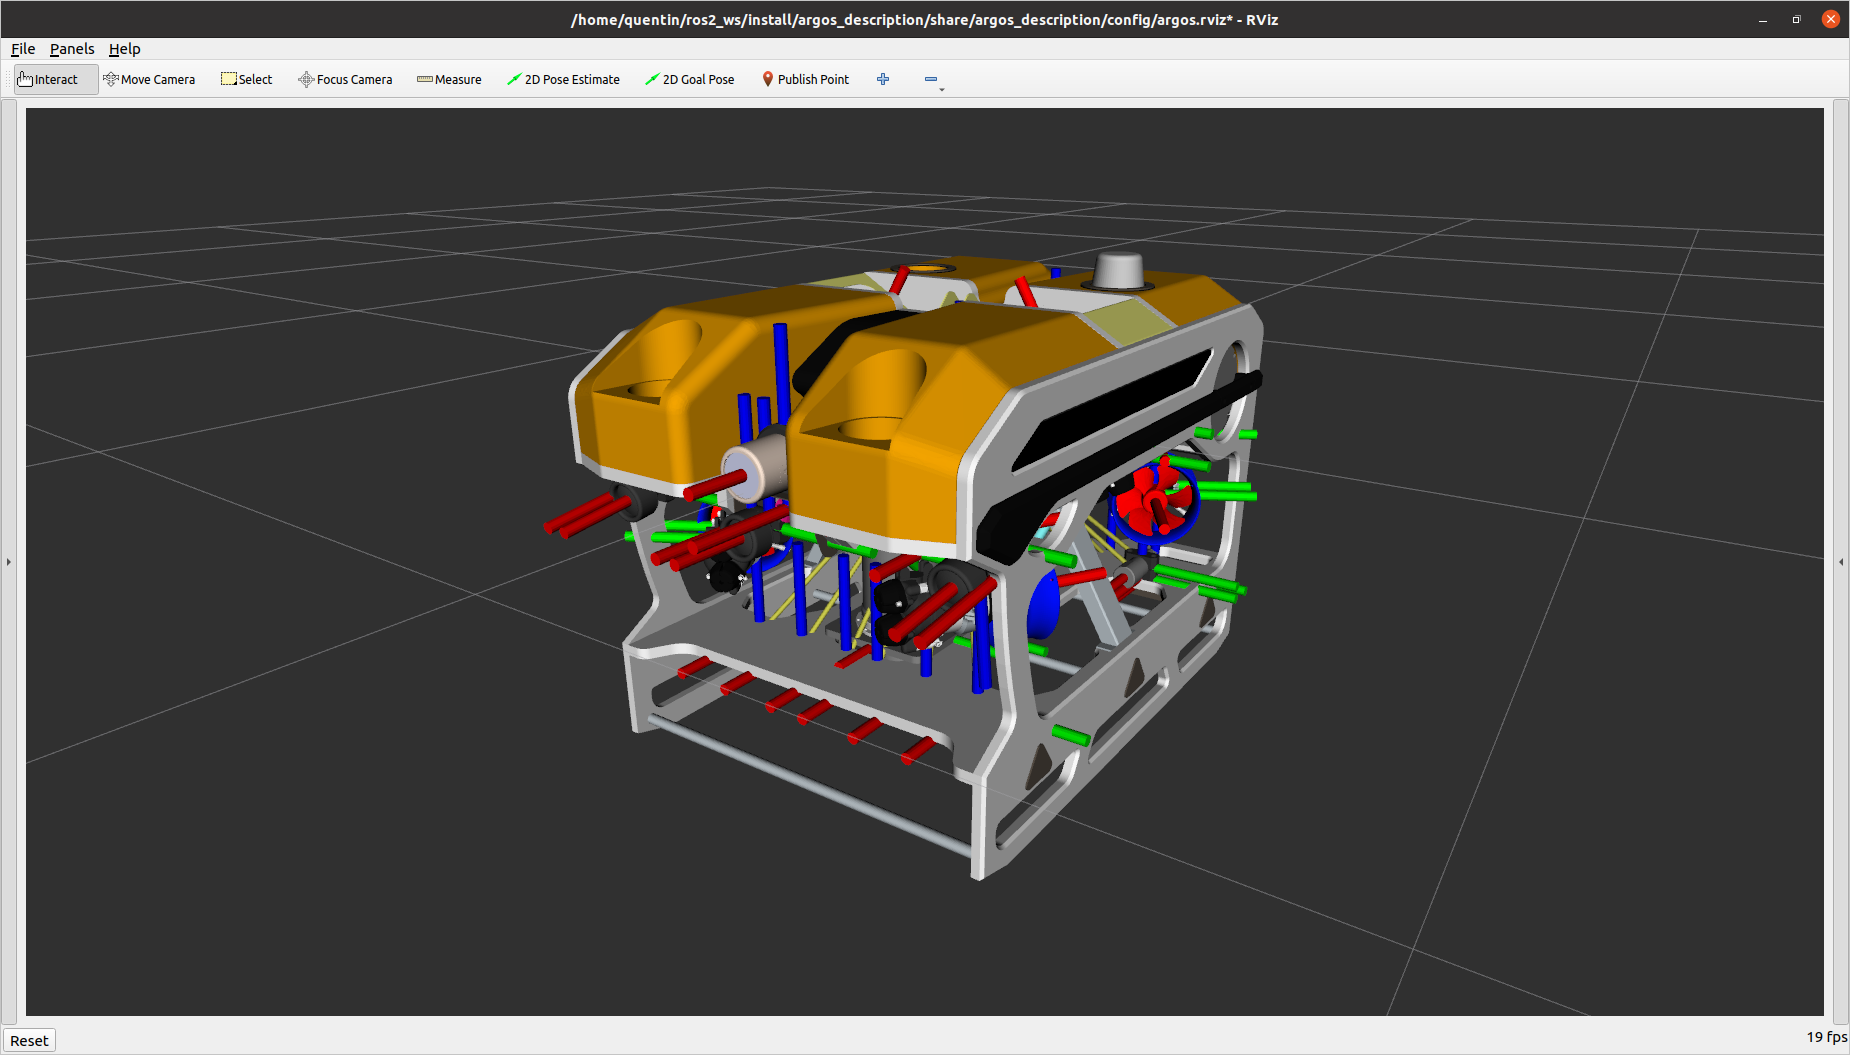
\includegraphics[width=\textwidth]{imgs/argos_rviz.png}
					\caption{\argos{} dans \textit{RViz2}}
					\label{fig:argos_rviz}
				\end{subfigure}
				\begin{subfigure}[t]{0.45\textwidth}
					\centering
					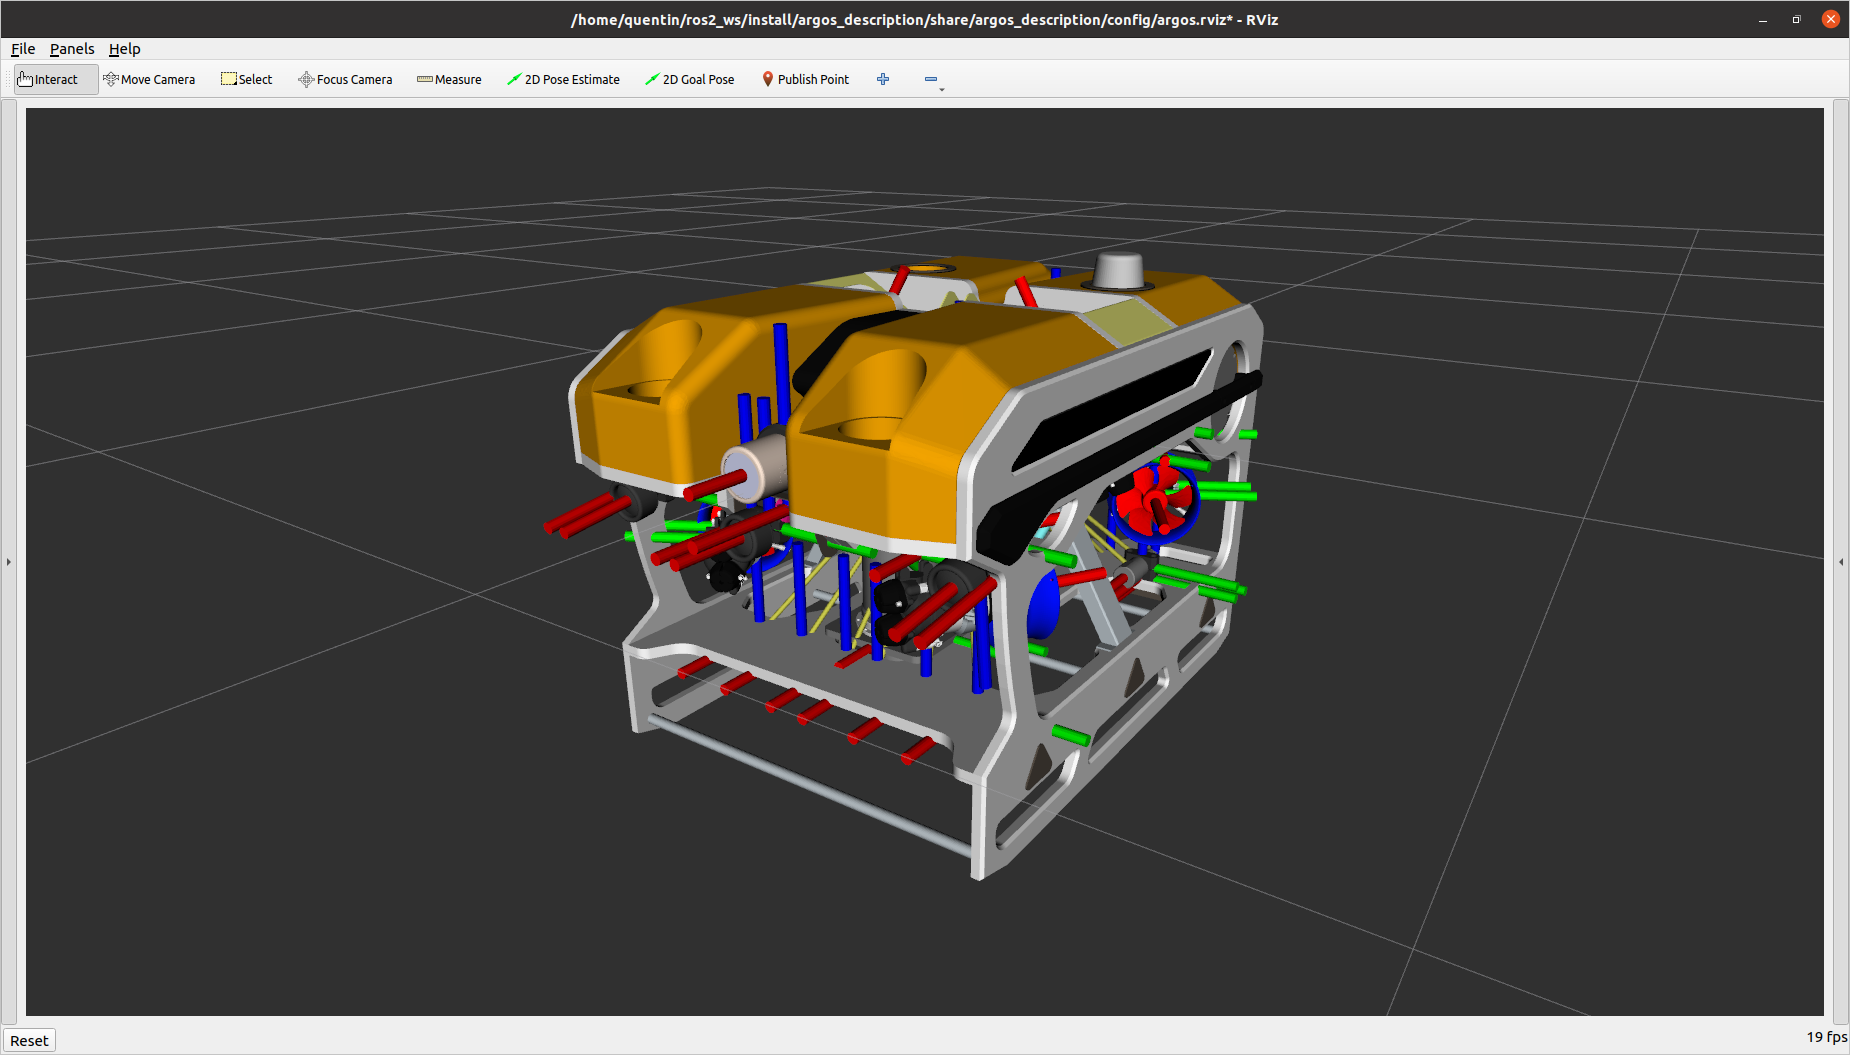
\includegraphics[width=\textwidth]{imgs/argos_rviz.png}
					\caption{\atoll{} dans \textit{RViz2}}
					\label{fig:atoll_rviz}
				\end{subfigure}
				\caption{Visualisation des robots dans \textit{RViz2}}
				\label{fig:rviz2_robots}
			\end{figure}

		\subsection{Invocation des robots dans l'environnement de simulation}

			Le premier test à réaliser est sûrement d'invoquer les robots dans le monde sous-marin afin de tester l'interaction des robots avec leur milieu. Il faut que le robot ait un comportement physique avec l'environnement de simulation qui soit acceptable. Globalement le robot doit avoir une flottabilité quasiment nulle, mais légèrement positive, afin qu'il remonte naturellement en cas de problème avec les propulseurs.

			On vérifie que les robots sont bien 

	\section{Comparaison avec les robots réels}

		Ecarts (statique/dynamique) lors d'essais en bassins ou réels

		\subsection{Rosace d'\argos{}}

			\argos{} a réalisé durant un essai des aller-retours avec une rotation de 3 degrés à chaque fois qu'il faisait demi-tour. Nous avons placé le robot à 10 mètres sous la surface afin de ne pas être impacté ni par les vagues ni par l'ombilical. Le mouvement dans le repère du monde ressemble globalement à des aller-retours entre deux points, mais si on trace la trajectoire dans le repère d'\argos{} on obtient une rosace. Cet essai a permis de tester le mouvement du robot dans son plan transverse suivant une multitude d'angles de déplacement par pas de 3 degrés et sur un espace restreint dans le repère du monde.

			\begin{figure}[!htb]
				\centering
				\begin{subfigure}[t]{0.48\textwidth}
					\centering
					\includegraphics[width=\textwidth]{build/imgs/rosace_global.pdf}
					\caption{Dans le repère du monde}
				\end{subfigure}
				\hfill
				\begin{subfigure}[t]{0.48\textwidth}
					\centering
					\includegraphics[width=\textwidth]{build/imgs/rosace_local.pdf}
					\caption{Dans le repère d'\argos{}}
				\end{subfigure}
				\caption{Rosace réalisée par Argos}
				\label{fig:rosace_argos}
			\end{figure}

	\section{Conclusion}